\documentclass[11pt,a4paper]{article}
\usepackage[T1]{fontenc}
\usepackage[utf8]{inputenc}
\usepackage{lmodern,microtype}
\usepackage[a4paper,left=24mm,right=24mm,top=24mm,bottom=24mm,headheight=14pt]{geometry}
\usepackage{amsmath,amssymb,amsthm,mathtools,array,booktabs,tabularx,enumitem,xcolor,fancyhdr}
\usepackage{tikz}
\usepackage[hyphens]{url}
\usepackage[colorlinks=true,linkcolor=black!70!blue,citecolor=blue!45!black,urlcolor=blue!45!black]{hyperref}
\definecolor{ink}{HTML}{193947}
\definecolor{teal}{HTML}{17645F}
\pagestyle{fancy}\fancyhf{}\fancyhead[L]{\small\sffamily\color{ink} Ehrhart zeros of symmetric edge polytopes}
\fancyhead[R]{\small\sffamily\color{ink} Keio and Shaitetsu}\fancyfoot[C]{\small\thepage}
\renewcommand{\headrulewidth}{0.3pt}
\newtheorem{theorem}{Theorem}[section]
\newtheorem{proposition}[theorem]{Proposition}
\newtheorem{corollary}[theorem]{Corollary}
\newtheorem{lemma}[theorem]{Lemma}
\theoremstyle{definition}\newtheorem{problem}[theorem]{Problem}
\setlist{topsep=4pt,itemsep=2pt}
\setlength{\emergencystretch}{2em}\allowdisplaybreaks[1]
\newcommand{\arxiv}[1]{\href{https://arxiv.org/abs/#1}{arXiv:#1}}
\newcommand{\doi}[1]{\href{https://doi.org/#1}{doi:#1}}
\hypersetup{pdftitle={From a line to a strip: Ehrhart zeros of symmetric edge polytopes},pdfauthor={Keio and Shaitetsu}}
\title{\color{ink}\bfseries From a line to a strip\\[3pt]\Large Ehrhart zeros of symmetric edge polytopes}
\author{Keio and Shaitetsu}
\date{Research manuscript \enspace$\cdot$\enspace 20 November 2026}
\begin{document}
\maketitle
\begin{abstract}
Higashitani, Kummer and Micha\l{}ek conjectured that the Ehrhart zeros of complete multipartite symmetric edge polytopes lie on the line $\Re x=-1/2$ and interlace under reduction of a largest part. We give exact counterexamples to both assertions. The smallest failure of the first occurs on twelve vertices. Even complete graphs with a matching removed have the entire strip $-1\le\Re x\le0$ as their set of finite limiting zeros. If the matching size grows as $\kappa d^\alpha$, with $1/2<\alpha\le1$, its rate selects exactly three limiting vertical lines. The proof starts from an optimal transport problem on a graph join. Its solution gives a pointwise identity for the polytope, a closed formula for all complete multipartite $\gamma$-coefficients, and the exact $\gamma$-degree of every nontrivial join. The degree formula also proves the conjectured characterization of vanishing $\gamma_k$ for all $k$-connected graphs with disconnected complement.
\end{abstract}

\section{The two assertions and the limiting zeros}
For a finite connected simple graph $G$ on $N$ vertices, take the lattice
$\Lambda=\{b\in\mathbb Z^N:\sum_v b_v=0\}$. Put
\[
 P_G=\operatorname{conv}\{\pm(e_u-e_v):uv\in E(G)\},\qquad
 E_G(m)=|mP_G\cap\Lambda|\quad(m\in\mathbb Z_{\ge0}).
\]
The edge differences of a spanning tree form a lattice basis, so the dimension is $d=N-1$. We use $E_G(x)$ for the unique degree-$d$ polynomial extending the counts. These polytopes are reflexive in $\Lambda$. In particular $E_G(-1-x)=(-1)^dE_G(x)$ and the numerator $h^*_G$ in $\sum_{m\ge0}E_G(m)t^m=h^*_G(t)/(1-t)^{d+1}$ is palindromic of degree $d$ \cite[Section~2.1]{HKM}. Set $\mathrm{CL}=\{x:\Re x=-1/2\}$.

Conjecture~4.10 of Higashitani, Kummer and Micha\l{}ek \cite{HKM} has two assertions. Every zero of $E_{K_{a_1,\ldots,a_s}}$ belongs to $\mathrm{CL}$. Also, decreasing a largest part by one gives a pair of polynomials whose zeros alternate in height on $\mathrm{CL}$. The authors checked graphs up to ten vertices. K\"olbl subsequently proved further families and studied the reach of the existing interlacing recurrences \cite{Kolbl}. Our examples use these precise polytopes, the same lattice and the specified largest-part operation.

\begin{theorem}\label{th:counter}
The polynomial $E_{K_{3,3,3,3}}$ has exactly four zeros off $\mathrm{CL}$. Twelve is the minimum vertex count for a counterexample. Moreover $E_{K_{2,3,3,3,3}}$ and $E_{K_{2,2,3,3,3}}$ each have all their zeros on $\mathrm{CL}$, and their zeros fail to alternate.
\end{theorem}

For the limiting statement, remove $b$ disjoint edges from $K_{d+1}$, where $0\le b\le\lfloor(d+1)/2\rfloor$, and retain connected graphs. Write $E_{d,b}$ for the Ehrhart polynomial of this graph. The finite limit set of a family consists of all $x$ for which $z_n\to x$ for some zeros in dimensions $d_n\to\infty$.

\begin{theorem}\label{th:limit}
For all admissible matching sizes together the finite limit set of $E_{d,b}$ is exactly the strip $-1\le\Re x\le0$. For an admissible sequence $b_d\sim\kappa d^\alpha$, $1/2<\alpha\le1$, $\kappa>0$, it is exactly the union of the three lines
\[
 \Re x=-\alpha,\qquad \Re x=-\tfrac12,\qquad \Re x=\alpha-1.
\]
For odd $d$ and $b=(d+1)/2$, let $M_d$ count the zeros off $\mathrm{CL}$ with multiplicity. Then $M_d/\log d\to\infty$.
\end{theorem}

For example, deleting $\lfloor d^{3/4}/2\rfloor$ disjoint edges selects the lines with real parts $-3/4,-1/2,-1/4$. Deleting a perfect matching on an even number of vertices moves the two outer lines to $-1$ and $0$. These are assertions about limits as dimension grows. The finite witnesses in Theorem~\ref{th:counter} have independent rational certificates.

\begin{figure}[htb]
\centering
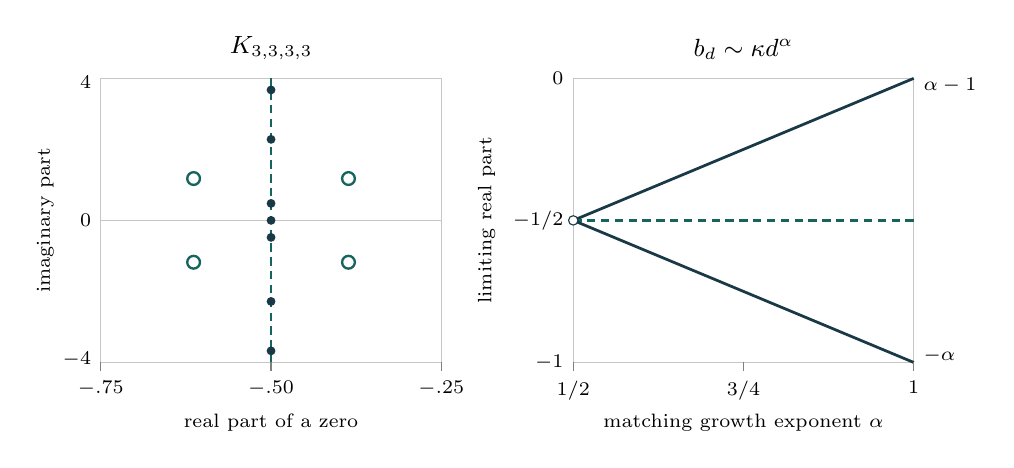
\begin{tikzpicture}[font=\small]
 \begin{scope}[x=.94cm,y=.44cm]
  \draw[gray!45] (0,-4.1) rectangle (4.6,4.1);
  \draw[gray!45] (0,0)--(4.6,0);
  \draw[teal,densely dashed] (2.3,-4.1)--(2.3,4.1);
  \foreach \y in {-3.765437,-2.339208,-.490005,0,.490005,2.339208,3.765437}
       \fill[ink] (2.3,\y) circle[radius=1.6pt];
  \foreach \x in {1.25374,3.34626}
       \foreach \y in {-1.207773,1.207773}
       \draw[draw=teal,fill=white,line width=.85pt] (\x,\y) circle[radius=2.3pt];
  \foreach \x/\t in {0/{-.75},2.3/{-.50},4.6/{-.25}}
       \draw[gray] (\x,-4.1)--(\x,-4.35) node[below,text=black] {\scriptsize $\t$};
  \foreach \y in {-4,0,4} \node[left] at (0,\y){\scriptsize $\y$};
  \node[above] at (2.3,4.35){\small $K_{3,3,3,3}$};
  \node[below] at (2.3,-5.3){\scriptsize real part of a zero};
  \node[rotate=90] at (-.75,0){\scriptsize imaginary part};
 \end{scope}
 \begin{scope}[shift={(6.0cm,0)},x=.94cm,y=.44cm]
  \draw[gray!45] (0,-4.1) rectangle (4.6,4.1);
  \draw[ink,line width=1pt] (0,0)--(4.6,4.1);
  \draw[teal,densely dashed,line width=.8pt] (0,0)--(4.6,0);
  \draw[ink,line width=1pt] (0,0)--(4.6,-4.1);
  \foreach \x/\t in {0/{1/2},2.3/{3/4},4.6/1}
        \draw[gray] (\x,-4.1)--(\x,-4.35) node[below,text=black] {\scriptsize $\t$};
  \foreach \y/\t in {-4.1/{-1},0/{-1/2},4.1/0} \node[left] at (0,\y){\scriptsize $\t$};
  \node[right] at (4.6,3.9){\scriptsize $\alpha-1$};
  \node[right] at (4.6,-3.9){\scriptsize $-\alpha$};
  \node[above] at (2.3,4.35){\small $b_d\sim\kappa d^\alpha$};
  \node[below] at (2.3,-5.3){\scriptsize matching growth exponent $\alpha$};
  \node[rotate=90] at (-1.17,0){\scriptsize limiting real part};
  \draw[draw=ink,fill=white] (0,0) circle[radius=1.7pt];
 \end{scope}
\end{tikzpicture}
\caption{Left, the eleven zeros in the first witness. Open circles mark its four off-line zeros. Plotted positions are rounded for display. Right, the real parts of the three lines of finite limiting zeros for each $1/2<\alpha\le1$. The excluded endpoint is open.}
\label{fig:zeros}
\end{figure}

\paragraph{How the arguments are related.}
The auxiliary problem is to minimize the mass transported along edges of a join with prescribed net flow at every vertex. A join has all edges between different factors. The optimum identifies points excluded by each factor, and the excluded regions are disjoint inside the complete-graph polytope. Lattice-point enumeration therefore reduces to one-factor corrections. For a missing matching the correction changes just one $\gamma$-coefficient. Its size controls the balance of two analytic terms with different powers of $d$. This balance supplies the off-line zeros. The same transport identity applied to matching supports gives an independent graph-theoretic application to \cite[Conjecture~3.13]{DJKV}.

\section{Optimal transport on a graph join}
Let $G=G_1\vee\cdots\vee G_s$ with $s\ge2$ on nonempty disjoint blocks $B_i$. Internal edges in each block are arbitrary. For a real zero-sum vector $b$ put $p_v=\max(b_v,0)$, $q_v=\max(-b_v,0)$ and $T=\sum_v p_v=\sum_v q_v$. Write $p_i,q_i$ for the totals on $B_i$. Let $\mu_i$ be the maximum mass transportable directly over internal edges of $G_i$ from supply to demand, with vertex capacities $p_v,q_v$. The gauge $\rho_G(b)=\inf\{t\ge0:b\in tP_G\}$ is the minimum total edge flow having imbalance $b$. This follows by expanding a point in $tP_G$ as a nonnegative combination of oriented edge vectors of total weight at most $t$, with unused weight assigned to $0$.

\begin{theorem}\label{th:join}
For every real $b$ of coordinate sum zero,
\[
 \rho_G(b)=\max\{T,\ \max_i(p_i+q_i-\mu_i)\}.
\]
Write $J_i=G_i\vee K_{N-|B_i|}$, on the same vertices as $G$. At every scale $m\ge0$ the indicator functions satisfy
\[
 {\bf1}_{mP_G}=\sum_{i=1}^s{\bf1}_{mP_{J_i}}-(s-1){\bf1}_{mP_{K_N}}. \tag{J}
\]
\end{theorem}

\begin{proof}
Use the bipartite graph of positive and negative vertices with the allowed direct edges of $G$. By capacitated max-flow/min-cut, the unmatched mass in a maximum direct transport is the maximum deficiency $p(S)-q(\mathcal N(S))$, over all subsets of sources (including the empty set). A set meeting two blocks reaches every demand vertex. For a nonempty subset of block $i$ all demands outside the block are reachable. The maximum internal deficiency, permitting the empty set, equals $p_i-\mu_i$ by the same cut formula on $G_i$. Thus the global deficiency is
\[
 \delta=\max\{0,\ \max_i(p_i-\mu_i-(T-q_i))\}.
\]
Allowing an empty set when computing the internal maximum cannot create a spurious positive deficiency, since $T-q_i\ge0$.

Every feasible flow decomposes into paths from supplies to demands and cycles. Discarding cycles and shortening paths can only reduce cost. At most $T-\delta$ mass can have cost one, and the remaining mass costs at least two per unit. Conversely, use a maximum direct transport and pair the unmatched masses. The endpoints of any such pair have distance at most two in a join. This attains cost $T+\delta$ and gives the gauge formula. With integral data the maximum direct transport and the pairing can be taken integral by flow integrality.

For the complete graph the gauge is $T$. In its $m$-dilate a violation $p_i+q_i-\mu_i>m$ requires $p_i+q_i>m$. At most one such violation can occur, since $\sum_i(p_i+q_i)=2T\le2m$. In $J_i$, only block $i$ can cause a violation, as all the other vertices can be viewed as singleton blocks. This proves (J) throughout the dilate. Outside it all indicators vanish.
\end{proof}

Summing (J) over $\Lambda$ gives the same linear identity for $E_G$. It also holds with any weight on the summed points. Since the dimension stays fixed, the same identity holds for $h^*$ and for the coefficients in its unique expansion
\[
 h_G^*(t)=\sum_{j=0}^{\lfloor d/2\rfloor}\gamma_j(P_G)t^j(1+t)^{d-2j},\qquad
 \gamma(P_G;z)=\sum_j\gamma_j(P_G)z^j .
\]
When all factors are edgeless, the formula reads $\rho_G(b)=\max(T,\max_i\sum_{v\in B_i}|b_v|)$. This gives two independent ways to compute the numerical witnesses below.

\section{Coefficients for complete multipartite graphs}
Let $G=K_{a_1,\ldots,a_h}$ with $h\ge2$ nonempty parts and $N=\sum a_i$. Binomial coefficients with an out-of-range lower index are zero. For $1\le j\le\lfloor(N-1)/2\rfloor$, define
\[
 F_j(a)=\sum_{s=j+1}^{2j}\binom{a}{s}\binom{N-1-a}{2j-s}.
\]
The full gamma expansion $h^*(P_G;z)=\sum_j\gamma_j z^j(1+z)^{N-1-2j}$ has $\gamma_0=1$ and
\[
 \gamma_j=\binom{2j}{j}\left(\binom{N-1}{2j}-\sum_{i=1}^h F_j(a_i)\right).\tag{P1}
\]
In particular every coefficient is nonnegative.

By (J), the loss in lattice points from the complete graph is the sum of individual block losses. This remains true for each $\gamma$-coefficient. For fixed $j\ge1$, let $d(a)$ denote the loss from one edgeless block of size $a$, divided by $\binom{2j}{j}$. We have $d(1)=0$.

Two known families determine $d$. The normalized gamma coefficients of $K_{a,b}$ and $K_{1,a-1,b}$, respectively, equal
\[
 \binom{a-1}{j}\binom{b-1}{j},\qquad
 \binom{a-1}{j}\binom{b}{j}.
\]
The first is \cite[Theorem~4.1]{HJM} and the second is \cite[Proposition~3.1(a)]{Kolbl}. Fix $b=N-a$ with $2\le a\le N-1$. Subtract the first family from the second. The unknown complete coefficient and the whole contribution of $b$ cancel, giving
\[
 d(a)-d(a-1)=\binom{a-1}{j}\binom{N-a-1}{j-1}.
\]
Now $F_j(a)$ counts the $2j$-subsets of an $(N-1)$-set having more than $j$ elements in a marked $a$-subset. Marking one more element creates exactly the displayed increment: the new subset contains that element, $j$ previously marked ones and $j-1$ from the remaining unmarked elements. Since $F_j(1)=0$, induction gives $d(a)=F_j(a)$. The star $K_{N-1,1}$ has zero gamma coefficient at $j\ge1$ by the bipartite formula. The normalized coefficient of the complete graph therefore equals $d(N-1)=\binom{N-1}{2j}$. Additivity proves (P1).

For a positive counting interpretation fix vertices $v,w$ in different parts and write $A$ for the part of $v$. Among $2j$-subsets of $V(G)\setminus\{v\}$ require at most $j$ elements in each part. Failure events for different parts are disjoint. Their individual counts are $F_j(a_i)$ except that $F_j(|A|-1)$ replaces $F_j(|A|)$ in the part of $v$ (with $F_j(0)=0$). Among the survivors remove those with exactly $j$ members of $A$ and containing $w$: this removes $\binom{|A|-1}{j}\binom{N-|A|-1}{j-1}=F_j(|A|)-F_j(|A|-1)$, since the total outside $A$ is then exactly $j$. The number left is precisely the bracket in (P1).

Let $a=\max_i a_i$. The cross-degree (the largest $j$ with $\gamma_j\ne0$) is exactly
\[
 \min\left(\left\lfloor\frac{N-1}{2}\right\rfloor,\ N-a-1\right).
\]
Indeed, choose the omitted vertex $v$ in a largest part $A$. Any counted subset of size $2j$ contains at least $j$ vertices outside $A$. At $j=N-a$ it would have to contain $w$ and saturate the bound in $A$, so only $j\le N-a-1$ is possible. For every $j\ge1$ satisfying both bounds, if $a-1\ge j$ one may take $j$ vertices in $A\setminus\{v\}$ and $j$ vertices outside $A$ avoiding $w$. If $a\le j$, every part automatically obeys the bound and $A\setminus\{v\}$ cannot saturate it, so any $2j$-subset works. This proves strict positivity throughout the asserted range.

\section{Exact certificates for the two counterexamples}
Write $v^+=\max(v,0)$ and $v^-=\max(-v,0)$. The membership formula yields
\[
 H_{a,m}(X,Y)=\sum_{\substack{v\in\mathbb Z^a\\\sum_i|v_i|\le m}}
                    X^{\sum_i v_i^+}Y^{\sum_i v_i^-},\qquad
 E_G(m)=\sum_{u=0}^m[X^uY^u]\prod_{j=1}^sH_{a_j,m}(X,Y).
 \tag{H}
\]
This formula applies to any number and sizes of parts. For explicit
integer arithmetic, the coefficient $[X^pY^q]H_{a,m}$ is zero for
$p+q>m$ and otherwise equals
\[
 \sum_{v=0}^{\min(a,p,q)}(-1)^v\binom av
       \binom{a+p-v-1}{a-1}\binom{a+q-v-1}{a-1},
\]
by expanding $((1-XY)/((1-X)(1-Y)))^a$. The dimension is $d=N-1$,
since the edge differences of a spanning tree span the zero-sum
hyperplane. Thus the first $d+1$ values in (H) determine the
entire Ehrhart polynomial through
$E_G(z)=\sum_{j=0}^d\binom zj\sum_{m=0}^j(-1)^{j-m}\binom jm E_G(m)$.

\paragraph{Failure of the canonical-line property.}
Take $G=K_{3,3,3,3}$. Formula (H) gives, in increasing order of $m$,
\begin{align*}
 E_G(0),\ldots,E_G(11)={}&1,109,3859,64351,643855,4478611,23785021,\\
                         &102685537,376512379,1210173327,3490713345,9198924405.
\end{align*}
The interpolation gives
\[
 E_G((-1+iz)/2)=-\frac{iz}{10218700800}Q(z^2),
\]
where
\begin{align*}
 Q(u)={}&83571u^5-7615685u^4+189849198u^3-1602884250u^2\\
       &+4965776431u-3452491665 .
\end{align*}
In ascending coefficient order, the signs of
$(1+y)^5Q(6y/(1+y))$ are $-,+,+,+,+,+$, and those of $Q(6+y)$
are $+,+,+,+,-,+$. Descartes' rule bounds the numbers of roots in
$(0,6)$ and $(6,\infty)$ by one and two respectively, with multiplicity.
Neither $0$ nor $6$ is a root. Thus $Q$ has at most three positive
roots; the canonical-line assertion would require five. In fact
$Q(0)<0<Q(1)$, $Q(21)>0>Q(22)$, and $Q(56)<0<Q(57)$,
and all the coefficients of $Q(-u)$ are negative. Consequently
exactly four roots of the degree-eleven polynomial $E_G$ are off
the canonical line.

\paragraph{Failure of interlacing on the canonical line.}
Let $G=K_{2,3,3,3,3}$ and $G'=K_{2,2,3,3,3}$, so $G'$ is obtained
by decreasing a largest part of $G$. Equation (H) and interpolation give
\[
 E_G((-1+iz)/2)=\frac{iz}{6376469299200}A(z^2),\qquad
 E_{G'}((-1+iz)/2)=\frac{1}{163499212800}B(z^2),
\]
where
\begin{align*}
 A(u)={}&1278059u^6-203796502u^5+9911355597u^4-177499861396u^3\\
       &+1199300771669u^2-3053747869302u+1935804366675,\\
 B(u)={}&220013u^6-27129498u^5+972506139u^4-12127443724u^3\\
       &+54197184723u^2-80729265978u+15445462725 .
\end{align*}
Direct substitution gives one sign change between the endpoints of each
of these disjoint intervals for its indicated polynomial:
\[
\begin{array}{c|rrrrrr}
 A &(0,1)&(22/5,5)&(5,6)&(18,19)&(42,43)&(87,88)\\
 B &(0,1)&(2,3)&(4,22/5)&(12,13)&(32,33)&(71,72).
\end{array}
\]
In each row the endpoint signs are $(+,-)$ in odd columns and $(-,+)$ in even columns. This accounts for
all six roots, each simple and positive. Both Ehrhart polynomials
therefore have only canonical-line roots. Among the positive
$z<\sqrt{22/5}$, the degree-thirteen polynomial has one root
and the degree-twelve polynomial has three. An alternating pair
can differ by at most one in its root counts on any interval. Hence
these two polynomials fail the proposed interlacing.

\paragraph{Minimal order of a counterexample to the root-location assertion.}
The smallest order is twelve. There are exactly two connected complete multipartite isomorphism types of this order that fail the canonical-line property: $K_{3,3,3,3}$ and $K_{2,2,2,2,2,2}$. The following is an independent exact census using the gamma formula; the preceding counterexample by itself suffices for disproof.
\[
\begin{array}{c|rrrrrrrrrrr}
N&2&3&4&5&6&7&8&9&10&11&12\\\hline
\text{profiles}&1&2&4&6&10&14&21&29&41&55&76\\
\text{profiles on the canonical line}&1&2&4&6&10&14&21&29&41&55&74
\end{array}
\]
Here a profile is a nondecreasing integer partition of $N$ into at least two parts. It determines the graph up to isomorphism, since its parts are the vertex classes in the complement. For reproducibility, use the following finite algorithm with integer polynomial products and ordinary division over $\mathbb Q$.

\begin{enumerate}
\item For each $N=2,\ldots,12$, generate profiles recursively by appending an integer $a$ from the previous part (initially $1$) through the unassigned sum, and recurse with that sum reduced by $a$. Keep complete partitions of length at least two. Put $d=N-1$.
\item Compute $h_i=[t^i]\sum_j\gamma_jt^j(1+t)^{d-2j}$ from the multipartite gamma formula. Form
\[
 F(Y)=\sum_{i=0}^d h_i\prod_{u=1}^d(Y+2u-2i-1).
\]
The binomial basis for Ehrhart polynomials gives $F(Y)=2^d d!\,E_G((Y-1)/2)$. Its coefficient $f_k=[Y^k]F(Y)$ vanishes unless $k\equiv d\pmod 2$. Set $Q(X)=\sum_{k\equiv d\ (2)}(-1)^{(d-k)/2} f_kX^k$. Thus $Q(X)=i^{-d}F(iX)$, and $E_G$ has canonical-line roots exactly when $Q$ has only real roots.
\item Start $S_0=Q,S_1=Q'$ and append $S_{i+1}=-\operatorname{rem}(S_{i-1},S_i)$ until the remainder is zero. Let $S_\ell$ be the last nonzero polynomial. For each $\eta\in\{-1,1\}$ let $v_\eta$ be the number of successive sign changes among $\eta^{\deg S_i}\operatorname{sgn}(\operatorname{lc}S_i)$, $i=0,\ldots,\ell$. Count the profile as on the canonical line precisely if $v_{-1}-v_1=d-\deg S_\ell$. Indeed Sturm's theorem counts distinct real roots, and $S_\ell$ is a scalar multiple of $\gcd(Q,Q')$, so the right side is the total number of distinct complex roots.
\end{enumerate}

\section{Limits under matching deletion}
For integers $d\ge1$ and $0\le b\le\lfloor(d+1)/2\rfloor$, let $E_{d,b}(x)$ be the Ehrhart polynomial of the symmetric edge polytope of $K_{d+1}$ with a matching of size $b$ removed, restricting to connected graphs. Its multipartite classes have sizes one and two. 

\paragraph{Existence and localization.} The set of finite limiting zeros of the polynomials $E_{d,b}$ contains the entire closed strip $-1\le\Re x\le0$. More precisely, fix $1/2<\alpha\le1$, $\kappa>0$, and a real $\tau\ne0$. Whenever $b_d\sim\kappa d^\alpha$ is an admissible sequence, for every sufficiently large $d$ there is a zero
\[
 x_d=\alpha-1+i\tau+O(1/\log d).
\]
The statement also holds on dimension subsequences. In particular, for every sufficiently large all-doubleton graph one can choose an Ehrhart zero, with the chosen zeros tending to $i$ as the number of parts grows.

Write $F_d(x)=E_{d,0}(x)$ and let $C_d(x)$ be the Ehrhart polynomial of the $d$-dimensional cross-polytope, whose Ehrhart series is $(1+z)^d/(1-z)^{d+1}$. Formula (P1) gives a loss of $2b$ in $\gamma_1$ and zero loss at every other index. The single-edge loss also appears in \cite[Example~5.7]{CRV}. Since $(1+z)^2-(1-z)^2=4z$, this yields the polynomial identity
\begin{equation}
 E_{d,b}(x)=F_d(x)-\frac b2\bigl(C_d(x)-C_{d-2}(x)\bigr)\qquad(d\ge2).
 \tag{L1}
\end{equation}
For the complete graph, (P1) gives $\gamma_j=\binom d{2j}\binom{2j}j$. The corresponding $h^*$ is $\sum_i\binom di^2 z^i$ by taking the constant term in $u$ of $(1+\sqrt z\,u)^d(1+\sqrt z/u)^d$. Thus
\[
 F_d(x)=\sum_{j=0}^d\binom dj\binom{d+j}j\binom xj,
 \qquad C_d(x)=\sum_{j=0}^d 2^j\binom dj\binom xj.
\]
Indeed, the generating function in the lattice dilation for $\binom xj$ is $z^j/(1-z)^{j+1}$. For the first formula the resulting coefficient of $\binom xj$ is $\sum_i\binom di^2\binom{d-i}{j-i}=\binom dj\binom{d+j}j$. For the second it is $2^j\binom dj$. Summing instead on the dimension $d$ gives
\begin{align}
 \sum_{d\ge0}F_d(x)s^d&=\frac1{1-s}
 {}_2F_1\left(-x,\tfrac12;1;\frac{-4s}{(1-s)^2}\right),\tag{L2}\\
 \sum_{d\ge0}C_d(x)s^d&=\frac{(1+s)^x}{(1-s)^{x+1}}.\tag{L3}
\end{align}
For (L2) use $\sum_{d\ge j}\binom dj\binom{d+j}j s^d=\binom{2j}j s^j/(1-s)^{2j+1}$. All powers denote their branches from $s=0$.

Fix $x_0=\delta+i\tau$ with $-1/2<\delta\le0$ and $\tau\ne0$. Uniformly for $x$ in a sufficiently small closed disk about $x_0$ one has
\begin{align}
 F_d(x)&=\frac{d^{2x}}{\Gamma(1+x)^2}
 +O\!\left(d^{2\Re x-1}+d^{-2\Re x-2}\right),\tag{L4}\\
 C_d(x)-C_{d-2}(x)&=\frac{2^{x+1}d^{x-1}}{\Gamma(x)}
 +O\!\left(d^{\Re x-2}+d^{-\Re x-2}\right).\tag{L5}
\end{align}
Here are details keeping both singularities. In (L2) put $Z=-4s/(1-s)^2$. At $s=1$, the connection formula at $Z=\infty$ has two nonresonant terms with leading powers $(-Z)^x$ and $(-Z)^{-1/2}$. The second is regular at $s=1$ after division by $1-s$. The first gives
\[
 \frac{4^x\Gamma(x+\tfrac12)}{\sqrt\pi\,\Gamma(1+x)}
 (1-s)^{-1-2x}\bigl(1+O(1-s)\bigr).
\]
At $s=-1$, $1-Z=(1+s)^2/(1-s)^2$. The two local terms are analytic and $(1+s)^{1+2x}$ times an analytic function, respectively. These are the only possible singularities on the unit circle, since the preimages of $0,1,\infty$ under $Z$ on that circle are $-1$ and $1$. The connection formulas are the Gauss identities \cite[equations 15.8.2 and 15.8.4]{DLMF}. Coefficient transfer at $1$ and $-1$ gives (L4), using $[s^d](1-s)^{-u}=d^{u-1}/\Gamma(u)+O(d^{\Re u-2})$ and the gamma duplication formula. For (L5) the dimension generating function is $(1+s)^{x+1}(1-s)^{-x}$, by multiplying (L3) by $1-s^2$. Its coefficient contributions at $1$ and $-1$ give the two errors stated in (L5). For uniformity, shrink the parameter disk to avoid resonances. The local connection series and their analytic factors then converge uniformly there on fixed smaller disks in $s$. Both generating functions continue to a common slit neighbourhood of the closed unit disk with cuts outward at $1$ and $-1$, by the hypergeometric differential equation or directly from (L3). The usual two-singularity transfer contour therefore gives bounds with constants uniform on that parameter disk \cite[Theorem~VI.5]{FS}.

Take $\delta=\alpha-1$, $L=\log d$, and let $m_d$ be a nearest integer to $\tau L/(2\pi)$. Put $x=\delta+(2\pi i m_d+w)/L$. On each compact set of $w$ this tends uniformly to $x_0$ and $d^{x-\delta}=e^w$. Equations (L1), (L4), and (L5) yield
\[
 d^{-2\delta}E_{d,b_d}\!\left(\delta+\frac{2\pi i m_d+w}{L}\right)
 \longrightarrow
 \frac{e^{2w}}{\Gamma(1+x_0)^2}
 -\frac{\kappa\,2^{x_0} e^w}{\Gamma(x_0)}
\]
locally uniformly. For instance the two error terms from $s=-1$, after normalization, are $O(d^{-4\delta-2})$ and $O(d^{-2\delta-1})$, both tending to zero because $\delta>-1/2$. Both coefficients in the limit are nonzero. It has a simple zero at any logarithm of $\kappa 2^{x_0}\Gamma(1+x_0)^2/\Gamma(x_0)$. By Rouch\'e's theorem on a small circle about one such zero, the scaled polynomial has a zero inside that circle for all sufficiently large $d$. This proves the stated localization estimate. Taking $d$ odd and $b_d=(d+1)/2$ gives the all-doubleton statement. Finally, these polytopes are reflexive, so $E_{d,b}(-1-x)=(-1)^d E_{d,b}(x)$. Reflection supplies the other half of the asserted strip, and closure supplies its central line and its real segment.

\subsection{The finite limit sets for growing matchings}
Under the growth hypotheses on $b_d$ in Theorem~\ref{th:limit}, we now show that its finite limit set equals
\[
 \{x:\Re x=\alpha-1\}\ \cup\ \{x:\Re x=-1/2\}\ \cup\ \{x:\Re x=-\alpha\}.
\]
Allowing all matching sizes $0\le b\le\lfloor(d+1)/2\rfloor$, the finite limit set equals $\{x:-1\le\Re x\le0\}$.

In the open half-plane $\Re x>-1/2$, (L4)--(L5) give locally uniform asymptotics
\[
 d^{-2x}F_d(x)\longrightarrow\frac1{\Gamma(1+x)^2},\qquad
 d^{1-x}\bigl(C_d(x)-C_{d-2}(x)\bigr)\longrightarrow\frac{2^{x+1}}{\Gamma(x)}.
\]
Indeed the bounds already given yield these conclusions on every small compact disk avoiding the resonant real parameters. The same Gauss connection expansions apply about any such nonresonant $x$ in this half-plane. To include a resonant point choose a small circle within the half-plane whose boundary avoids all resonances. The two differences between the normalized functions and their claimed limits are holomorphic in the whole disk. Their boundary convergence gives uniform convergence on the disk by the maximum modulus principle. For $\Re x>\alpha-1$, the first term dominates in (L1), locally uniformly after division by $d^{2x}$, since $1/\Gamma(1+x)^2$ has no zeros there. For $-1/2<\Re x<\alpha-1$, division by $d^{x+\alpha-1}$ leaves the second term with nonvanishing limit $-\kappa 2^x/\Gamma(x)$. These open half-strips have no finite limits of zeros. Reflexivity excludes their reflections as well. The two outer lines occur by the localization estimate and the fact that a finite limit set is closed.

For the middle line fix $\tau\ne0$ and set $x=-1/2+it$ with $t$ in a small real interval about $\tau$. Retaining the leading coefficient at $s=-1$ together with that at $s=1$ in the proof of (L5) gives uniformly
\[
 C_d(x)-C_{d-2}(x)=d^{-3/2}\left(A(t)e^{it\log d}+(-1)^d\overline{A(t)}e^{-it\log d}\right)+O(d^{-5/2}),
 \quad A(t)=\frac{2^{x+1}}{\Gamma(x)}.
\]
At $s=-1$ the singular factor is $(1+s)^{x+1}$ and its analytic prefactor is $2^{-x}$; on this line $-1-x=\bar x$. The same connection calculation at both endpoints in (L2) gives $F_d(x)=O(d^{-1})$ there. The exponent differences are nonresonant since $t\ne0$. Thus the real function $i^{-d}E_{d,b_d}(-1/2+it)$, divided by $-b_d d^{-3/2}$, is
\[
 |A(t)|\cos\bigl(t\log d+\arg A(t)-\pi d/2\bigr)+o(1)
\]
uniformly on that interval, since $b_d/\sqrt d\to\infty$. Its realness follows from conjugation and reciprocity. Choose $t_1$ within $\pi/\log d$ of $\tau$ satisfying $t_1\log d+\arg A(\tau)-\pi d/2\in2\pi\mathbb Z$, and put $t_2=t_1+\pi/\log d$. Since $A$ has a continuous nonzero argument branch locally, the two displayed values have opposite signs for large $d$. The intermediate value theorem gives an actual canonical-line zero at distance $O(1/\log d)$ from $-1/2+i\tau$. Taking closure gives the midpoint $-1/2$ too. This proves the assertion for fixed growth. For example, admissible integer sequences may be chosen as $b_d=\min(\lfloor\kappa d^\alpha\rfloor,\lfloor(d+1)/2\rfloor)$ whenever $\alpha<1$, or when $\alpha=1$ and $\kappa\le 1/2$.

For arbitrary $b\le(d+1)/2$, the two locally uniform limits in $\Re x>0$ show directly that $d^{-2x}E_{d,b}(x)\to1/\Gamma(1+x)^2$ uniformly on its compact subsets, uniformly in the admissible matching size. Thus $\Re x>0$ and, by reciprocity, $\Re x<-1$ contain no finite limits. The localization estimate and reflection supply every point of the remaining closed strip.

\subsection{How many roots leave the canonical line?}
Let $d$ tend to infinity through odd integers, set $b=(d+1)/2$,
and let $M_d$ be the number of zeros of $E_{d,b}$ off the
canonical line, counted with multiplicity. Then
\[
                         \frac{M_d}{\log d}\longrightarrow\infty .
\]
More precisely, for every fixed $0<a<c$, at least
$(c-a)\log d/(2\pi)-O_{a,c}(1)$ distinct zeros lie at distance
$O_{a,c}(1/\log d)$ from the segment $i[a,c]$.

Put $L=\log d$, and on a fixed small neighbourhood of $i[a,c]$ set
\[
 A(x)=\frac1{\Gamma(1+x)^2},\qquad
 h(x)=\frac{2^{x-1}\Gamma(1+x)^2}{\Gamma(x)}.
\]
Both are nonvanishing there. On a simply connected smaller
neighbourhood fix an analytic logarithm $g=\log h$.
For each $k$ with $u_k=2\pi k/L\in[a,c]$ put
$x_k(w)=iu_k+(g(iu_k)+w)/L$.
Equations (L1), (L4), and (L5), uniformly on the compact segment
and bounded $w$-disks, yield
\[
 E_{d,b}(x_k(w))
   = A(iu_k)h(iu_k)^2 e^w(e^w-1)+o(1).
\]
Indeed $d^{x_k(w)}=h(iu_k)e^w$, and the error is uniform in $k$
by a finite covering of the segment by the parameter disks
in (L4)--(L5). For any fixed $0<\rho<\pi$, the leading expression
is bounded away from zero uniformly on $|w|=\rho$ and has one
simple zero inside. Rouch\'e's theorem supplies one zero in each
$x_k(\{|w|<\rho\})$. These disks are pairwise disjoint for large $d$:
the imaginary coordinates of consecutive centers differ by
$2\pi/L+O_{a,c}(L^{-2})$, since $g'$ is bounded near the segment.
The number of admissible $k$ proves the quantitative assertion.

For large $d$ these zeros have positive imaginary part and real part
close to zero. Complex conjugation and the reflection $x\mapsto-1-x$
produce three disjoint further sets near $-i[a,c]$ and
$-1\pm i[a,c]$. Hence
$\liminf_{d\to\infty} M_d/\log d\ge 2(c-a)/\pi$.
The segment length $c-a$ is arbitrary, proving the limit.

\section{Edge addition in a join factor}
For a graph $B$ on a fixed vertex set $W$, put $\widehat B=B\vee K_1$. For $2j\le |W|$, define $\mathcal M_j(B)$ to consist of the ordered pairs $(X,Y)$ of disjoint $j$-subsets of $W$ for which the edges of $B$ between $X$ and $Y$ admit a perfect matching. Each pair is counted once, irrespective of the number of matchings. Then
\[
 \gamma_j(P_{\widehat B})=|\mathcal M_j(B)|.
\]
This form of the suspension identity follows from Ohsugi and Tsuchiya~\cite[Theorem~3.1 and Proposition~4.1]{OTmatch}. In detail, choose a two-colouring of $W$ uniformly, and keep only its bichromatic edges. Their formula is $4^j$ times the expected number of $2j$-subsets supporting a perfect matching of this cut graph. A fixed ordered pair $(X,Y)$ in $\mathcal M_j(B)$ has all of $X$ red and all of $Y$ blue with probability $2^{-2j}$; all colours outside $X\cup Y$ are free. Summing over the ordered pairs gives the identity.

For clarity, independent vertex colours give the same conclusion for disconnected $B$. Its suspended components meet only at the common apex, so the block product for $h^*$~\cite[Proposition~5.2]{OTanti} gives the product of their $\gamma$-polynomials (their dimensions sum). The generating polynomial $\sum_j |\mathcal M_j(B)|z^j$ factors the same way: any perfect matching of a bichromatic induced support pairs vertices within each connected component. An isolated vertex contributes the constant polynomial $1$. Thus one may apply the connected identity componentwise without interpreting coincident cut edge sets as distinct graphs. In particular, for spanning graph inclusions $B\subseteq B'$ the inclusion $\mathcal M_j(B)\subseteq\mathcal M_j(B')$ proves coefficientwise edge monotonicity for suspensions.

Now let $G=G_1\vee\cdots\vee G_s$ on $N$ vertices, with $s\ge2$ and nonempty, pairwise disjoint vertex sets $A_i$. Write $J_i=G_i\vee K_{N-|A_i|}$, the graph obtained by keeping only the possibly missing edges within $A_i$. The preceding disjoint-defect valuation in fixed dimension gives
\[
 \gamma(P_G;z)=\sum_{i=1}^s\gamma(P_{J_i};z)-(s-1)\gamma(P_{K_N};z).
\]
If edges are added within $A_i$, the difference of the two sides is exactly the change of $\gamma(P_{J_i};z)$. A vertex outside $A_i$ is a universal vertex of $J_i$ before and after the change, so the suspension identity proves that the difference has nonnegative coefficients. Repeating this for each factor proves monotonicity for arbitrary spanning edge additions within the factors of a fixed join. In particular $\gamma(P_G;z)$ dominates coefficientwise the $\gamma$-polynomial for the complete multipartite graph on the parts $A_i$; the complete multipartite formula above proves coefficientwise nonnegativity on every nontrivial join.

We record the exact threshold at which a small factor cannot affect a coefficient. If $|A_i|\le j$ and $2j\le N-1$, then $\gamma_j(P_{J_i})=\gamma_j(P_{K_N})$. Choose a suspension apex outside $A_i$. For any pair $(X,Y)$ of disjoint $j$-subsets of the remaining vertices, the bipartite graph between $X$ and $Y$ has a perfect matching even when all internal edges of $A_i$ are absent. A subset of $X$ meeting the complement of $A_i$ sees all of $Y$. A subset of $X\cap A_i$ sees at least $j-|Y\cap A_i|\ge |X\cap A_i|$ vertices, since $|A_i|\le j$. Hall's theorem and the suspension identity prove the claim. For an edgeless $A_i$, a $2j$-element support with more than $j$ vertices in $A_i$ cannot be perfectly matched, since each vertex of $A_i$ needs a partner outside. With at most $j$ such vertices the same Hall argument works on that support. Counting its $\binom{2j}{j}$ colourings gives a second derivation of the individual deficit in (P1).

\section{Matching number and vanishing coefficients}
Let $G$ be a nontrivial join on $N$ vertices, and let $H$ be the subgraph induced by a largest connected component of its complement (that is, $H=G[A]$ for such a vertex set $A$). Set $r=N-|A|$, and write $\nu(H)$ for its maximum matching size. Then
\[
 \deg\gamma(P_G)=\min\!\left(\left\lfloor\frac{N-1}{2}\right\rfloor,\ r-1+\nu(H)\right),
\]
and every coefficient from index zero to this degree is strictly positive.

Indeed, take $1\le j\le\lfloor(N-1)/2\rfloor$. If $j<r$, the complete multipartite graph on the complementary components has positive $j$th coefficient, and within-factor edge monotonicity gives the assertion for $G$. Suppose $r\le j$. Every complementary component other than $A$ has at most $r\le j$ vertices. By the small-factor result just proved, each of their deficits at index $j$ vanishes.

Consequently $\gamma_j(P_G)=\gamma_j(P_{H\vee K_r})$. The suspension cut formula makes this coefficient positive exactly when $H\vee K_{r-1}$ has a matching of size $j$: any matching survives a colouring giving opposite colours to its ends, and a nonzero summand gives such a matching. At most $r-1$ of its edges can use the clique. Conversely, a matching of $j-r+1$ edges in $H$ extends to one of size $j$ by matching the $r-1$ clique vertices to unused vertices of $H$. There are enough since $N\ge 2j+1$. This gives the degree and support claim.

\paragraph{Application to a vanishing conjecture.} Conjecture~3.13 of D'Al\`i, Juhnke-Kubitzke, K\"ohne and Venturello \cite{DJKV} proposes a characterization of the vanishing of $\gamma_k$ for $k$-connected graphs. We prove their characterization for every graph with disconnected complement. Take $k\ge2$ and a $k$-connected join $G$ on $N\ge 2k+1$ vertices. The case $N<2k+1$ has $\gamma_k=0$ by degree. In the nontrivial range, $\gamma_k=0$ forces $r\le k$ and $\nu(H)\le \ell:=k-r$ by the degree formula. Deleting the $r$ vertices outside $A$ shows that $H$ has connectivity at least $\ell$ when $\ell>0$.

By the Tutte--Berge formula, there exists $S\subseteq A$ such that, writing $o$ for the number of odd-order components,
\[
 o(H-S)-|S|=|A|-2\nu(H)\ge |A|-2\ell\ge r+1\ge2.
\]
Thus $H-S$ is disconnected and $|S|\ge\ell$, also trivially if $\ell=0$. Since $o(H-S)\le |A|-|S|$, one has $|S|\le \nu(H)\le\ell$. It follows that $o(H-S)=|A|-|S|$, so $|S|=\ell$ and $H-S$ is independent. Each remaining vertex has degree at least $\ell$ in $H$ and is adjacent to all of $S$. Hence $S\cup(V(G)\setminus A)$ has size $k$ and is completely joined to an independent set of size $N-k$, as conjectured. Conversely, suppose $G$ is between $K_{k,N-k}$ and the join of $K_k$ with an independent set of size $N-k$, on the same bipartition. The independent side is a largest complementary component because $N-k>k$. Here $r=k$ and $\nu(H)=0$, so $\gamma_k=0$. This also proves the sufficient condition of the original conjecture without a separate hypothesis on the complement: every graph in the stated interval is automatically a join.

\section{Relation to earlier methods}
The corpus suggested two specific steps. Manuscript 225, in its lemma on exact flow distance in a vertex lattice, turns a polyhedral gauge into an optimization over coefficients. Manuscript 071, in its work on equivariant Ehrhart counterexamples, uses a tractable family and exact lattice information to certify failure in growing dimension \cite{Corpus}. Here a positive transport deficiency in a join arises inside a single block. This makes the correction additive at the level of indicator functions. The subsequent dimension asymptotics determine the locations and the number of zeros created by a growing matching.

Ohsugi and Tsuchiya proved an analogous one-factor subtraction formula for the $h^*$-polynomials of \emph{PQ-type adjacency polytopes} \cite[Theorem~1.1]{PQ}. Their points record both endpoints in two coordinate blocks, including diagonal pairs. The symmetric edge polytopes here use differences in one sum-zero lattice. Projection by subtraction maps the former vertices onto the latter polytope, and fibers affect lattice counts. For instance, on $K_2$ the PQ polytope is the product of two unit segments, whereas $P_{K_2}$ is a segment of lattice length two. Thus the two Ehrhart polynomials are $(m+1)^2$ and $2m+1$. Mori, Mori and Ohsugi studied facet counts on this same class of graph joins \cite{MMO}. Codenotti, Riccardi and Venturello explicitly evaluated the one-edge $h^*$ loss of the complete graph \cite[Example~5.7]{CRV}. Equation (J) explains exact superposition for disjoint missing edges, including after arbitrary further deletions inside separate join factors.

The nonnegativity of $\gamma$ on joins has a necessary scope qualification. Ferroni gives counterexamples among general symmetric edge polytopes \cite{Ferroni}. The matching argument for joins also gives coefficientwise monotonicity under edge additions, a property which can fail for general graphs \cite[Example~3.9]{DJKV}. The classification from Conjecture~3.13 proved here covers graphs with disconnected complement. The full resolution in this paper concerns both clauses of the earlier root conjecture \cite{HKM}.

\paragraph{Literature status.}
The original 2016 preprint and 2017 article, K\"olbl's 2024 paper and 2025 dissertation, and the sources on graph joins, matching supports and edge deletion above were compared with the two counterexamples. Searches by conjecture number, graph families, matching deletions and author citations located special positive cases and the single-edge formula. We did not locate an earlier disproof of Conjecture~4.10, or the same finite limit set for these graphs. This records the scope of the priority check as of 20 November 2026. Historical priority and external peer review remain unverified.

\begin{thebibliography}{99}\small
\bibitem{HKM} A.~Higashitani, M.~Kummer and M.~Micha\l{}ek.
Interlacing Ehrhart polynomials of reflexive polytopes.
\emph{Selecta Math. (N.S.)} \textbf{23} (2017), 2977--2998.
\arxiv{1612.07538}. \doi{10.1007/s00029-017-0350-6}.
\bibitem{Kolbl} M.~K\"olbl. On a conjecture concerning the roots of Ehrhart polynomials of symmetric edge polytopes from complete multipartite graphs (2024). \arxiv{2404.02136}.
See also Chapter~5 of \emph{Enumerative and algebraic invariants of lattice polytopes}, doctoral dissertation, The University of Osaka (2025). \doi{10.18910/101775}.
\bibitem{HJM} A.~Higashitani, K.~Jochemko and M.~Micha\l{}ek.
Arithmetic aspects of symmetric edge polytopes.
\emph{Mathematika} \textbf{65} (2019), 763--784.
\doi{10.1112/S0025579319000147}.
\bibitem{OTmatch} H.~Ohsugi and A.~Tsuchiya. Symmetric edge polytopes and matching generating polynomials.
\emph{Combinatorial Theory} \textbf{1} (2021), paper 9. \doi{10.5070/C61055371}.
\bibitem{OTanti} H.~Ohsugi and A.~Tsuchiya. The $h^*$-polynomials of locally anti-blocking lattice polytopes and their $\gamma$-positivity. \emph{Discrete Comput. Geom.} \textbf{66} (2021), 701--722. \doi{10.1007/s00454-020-00236-6}.
\bibitem{PQ} H.~Ohsugi and A.~Tsuchiya. PQ-type adjacency polytopes of join graphs. \emph{Discrete Comput. Geom.} \textbf{70} (2023), 214--235.
\doi{10.1007/s00454-022-00447-z}.
\bibitem{MMO} A.~Mori, K.~Mori and H.~Ohsugi. Number of facets of symmetric edge polytopes arising from join graphs. \emph{European J. Combin.}, article 104165. \doi{10.1016/j.ejc.2025.104165}.
\bibitem{DJKV} A.~D'Al\`i, M.~Juhnke-Kubitzke, D.~K\"ohne and L.~Venturello.
On the gamma-vector of symmetric edge polytopes.
\emph{SIAM J. Discrete Math.} \textbf{37} (2023), 487--515. \doi{10.1137/22M1492799}.
\bibitem{CRV} G.~Codenotti, R.~Riccardi and L.~Venturello. The number of edges of a symmetric edge polytope. \arxiv{2512.16572}, version 2 (2026).
\bibitem{Ferroni} L.~Ferroni. Symmetric edge polytopes are not gamma-positive. \arxiv{2607.02424} (2026).
\bibitem{FS} P.~Flajolet and R.~Sedgewick. \emph{Analytic Combinatorics}. Cambridge University Press, 2009, Chapter~VI, Theorem~VI.5. \doi{10.1017/CBO9780511801655}.
\bibitem{DLMF} NIST Digital Library of Mathematical Functions. Chapter~15, Hypergeometric function, \S15.8(i). \url{https://dlmf.nist.gov/15.8}.
\bibitem{Corpus} QEEDDD. \emph{Verifiable Mathematical Reasoning Corpus}. Manuscripts 071 and 225, snapshot \texttt{c2ac34ea4622}. \href{https://github.com/QEEDDD/Verifiable-Mathematical-Reasoning-Corpus/tree/c2ac34ea4622778187173f41bb1996deee8081b7}{Archived repository revision}.
\end{thebibliography}
\end{document}
